% !TEX root ../thesis
\chapter{Related work\label{ch:Related_work}}

\abstract{This chapter introduces related work both on \glspl{bn} (especially \gls{p2p} based) in general as well as specifically on Dridex.
Furthermore, it provides a short introduction to the process of reverse engineering and counter-measures to it.}

\section{Botnets\label{sec:Related_work::Botnets}}
\Glspl{bn} can be divided into two major categories based on their architecture: centralized and distributed.
Both types come with tradeoffs regarding ease of development and resilience.

\paragraph*{Centralized architectures}
Simple \glspl{bn} use a single \gls{c2} server to control the infected machines.
Popular choices include \gls{irc} and plain \gls{http} based web servers which expose endpoints for the \glspl{bot} to connect to~\cite{aburajab2006multifaceted}.
The \gls{mw}'s code contains a hardcoded \gls{ip} address (and port) to connect to where the communication backend is hosted.
This architecture trades stability for ease of development and is very vulnerable to takedown attempts.
If the controlling server (or even multiple servers) are taken offline, the \glspl{bot} are no longer a direct threat as no new commands from the \gls{c2} will be received.

To mitigate this single-point-of-failure, multiple approaches exist.
\emph{Mirai}, an \gls{iot} worm used to perform powerful \gls{ddos} attacks, uses domain names instead of hardcoded \gls{ip} addresses to identify its \gls{c2} server.
This enables the \gls{bm} to dynamically switch out the contacted server by modifying the corresponding \acrshort{dns} entry.
Combined with a short \gls{ttl} this solution provides a responsive protection against regular takedown attempts while maintaining relatively low complexity.

However, \gls{dns} based control structures expose other potential weaknesses limiting the \gls{mw} spread.
In 2009 the Spanish based \gls{bn} called \emph{Mariposa} was taken down by \emph{sinkholing} the \gls{c2} domains used to control the \glspl{bot}.
Security operators seized the set of domains in a collaborative effort with domain registrars and law enforcement across several different countries effectively halting all \gls{bn} communication~\cite{krebs2010mariposa, nadji2013beheading}.
To prevent sinkholing, \gls{dns} based \gls{mw} started to transition from hardcoded domain names to \glspl{dga}.
These algorithms include certain environmental factors such as date and time or system language to generate a huge list of potential \gls{c2} domain names.
The \gls{bot} then initiates connections to these domains until one correctly resolves and responds in the correct protocol.
Popular examples such as Conficker-C generated about 50.000 names per day hindering effective sinkholing massively~\cite{porras2009conficker}.
But as the \gls{dga} has to be used in the \gls{mw} it has to be included in the binary and as such can be reverse engineered.
This allows security professionals to predict future results and include the domains in blacklists for example in firewalls or \gls{ids}.

The transition from single hardcoded servers to \gls{dga} based structures increases the robustness of centralized \glspl{bn} massively and makes takedown attempts a lot less likely to succeed completely.
However there are still ways to partially mitigate the impact of \glspl{bn} through netflow analysis and \gls{ids}.


\paragraph*{Distributed architecture}
To avoid \gls{dns} based problems multiple \glspl{bn} have transitioned to \gls{p2p} protocols~\cite{dittrich2008new}.
Instead of a defined \gls{c2} (via \gls{dns} or \gls{dga}) each \gls{bot} now maintains a \emph{\gls{pl}} filled with information about other \glspl{bot} it can connect to.
The \glspl{bm} can issue commands through a selection of special \glspl{bot} which they control directly.
The protocol then ensures these commands are populated and executed throughout the \gls{bn}.
This makes complete disruption of the communication immensely hard as the size of each bot's \gls{pl} can easily reach 1000 and more~\cite{haas2016resilience}.

An important concept in \gls{p2p} networks in general and \gls{p2p} \glspl{bn} especially is the notion of so-called \emph{\glspl{sp}}.
While a regular server is often directly connected to the internet, \glspl{bot} are mostly infected consumer or office machines which are separated from the public address space via firewalls or behind a \gls{nat} device.
This limits their capabilities in the \gls{p2p} network as connections are usually limited to be outbound to other peers, while incoming requests are filtered or blocked.
As connectivity of all \glspl{bot} is the main goal of a \gls{p2p} \gls{bn} it requires some peers to have a publicly routable \gls{ip} address to accept connections from infected hosts behind \gls{nat}.
These \glspl{sp} represent a significantly lower percentage of the total network peers but are invaluable in keeping the network connected.
Rossow et al.\ estimate that only around 13--40\% of the total peers of a \gls{bn} are \glspl{sp}~\cite{rossow2013sok}.
This makes them an ideal target for takedown attempts.


\paragraph*{\gls{p2p} \gls{bn} monitoring}
It is very important to study a \gls{bn} over long periods of time to gain insight about its reach and growth.
Following the evolution from centralized \glspl{bn} to \gls{p2p} networks the security community had to adapt and evolve monitoring techniques.
Since \gls{p2p} \glspl{bn} constantly change when new \glspl{bot} enter or leave the network (this is called \gls{node_churn}), obtained results are quickly outdated or inaccurate.
As a result, monitoring has to be resilient, long-running, and mostly automated to continually gather information.
Main objective is to obtain information about the \emph{full population} (total number of active peers) of a \gls{bn} to estimate its capabilities in regards to computing power and bandwidth.
To achieve this in a \gls{p2p} context, two major approaches exist: \emph{crawling} and \emph{sensor injection}.
\begin{description}
    \item[Crawling]
    A \gls{bn} \gls{crawler} captures data about active \glspl{sp} of the network by continuously requesting the \glspl{pl} of known \glspl{bot} and enumerating them.
    This approach generates a view on the \gls{bn} from the perspective of a regular peer as the online status of non-\glspl{sp} cannot be verified limiting its usefulness in regards to population levels.
    \item[Sensor injection]
    To gain insights from the perspective of a \gls{sp} a \gls{sn} can be injected into the network.
    This node implements the \gls{bn} protocol and acts as fake \gls{sp} similar to a \gls{hp}.
    This approach can be used to verify connections originating from \glspl{bot} behind \gls{nat} and usually produces a more realistic view over the number of active peers.
\end{description}

Unfortunately most major \glspl{bn} employ some method of protection against intelligence gathering and are constantly adapted to limit or block the use of the aforementioned techniques~\cite{rossow2013sok, yan2011ratbot}.


\section{Dridex\label{sec:Related_work::Dridex}}
Dridex is currently one of the most dangerous financial trojans.
Its primary focus is credential theft of online banking sites but it also includes components for remote control of infected machines through \gls{vnc}.
Dridex is the successor of the famous Cridex worm, adding a \gls{p2p} network layer and switching from self-propagation to spam emails as the main distribution vector.
Since its inception in 2014, the \gls{mw} has been constantly updated, to avoid detection by antivirus software and explore new ways to infect targets~\cite{ramos2016dridex, proofpoint2017dridex, teo2015learning, tokazowski2016dridex}.
Internally Dridex is divided into multiple \emph{subnets} which are most likely controlled by different teams with each subnet often focussing on single countries or regions.

While other infection vectors are often explored, spam email campaigns remain the main distribution mechanism of Dridex.
These emails are highly customized targetting a selected country or even a single company and contain malicious attachments often disguised as trustworthy messages such as scanned documents or invoices.
The attached files are mostly Microsoft Office documents or script files with a fake extension which download and launch Dridex.
The user is then tricked into enabling macro execution by a message stating that the document cannot be displayed correctly without them.
Although this behavior is common among phishing emails, Dridex's spam campaigns are of an unusually high quality with very few spelling errors and convincing domain names.
The level of professionalism hints that the organization behind Dridex is highly experienced~\cite{obrien2016dridex}.

\begin{figure}
    \centering
    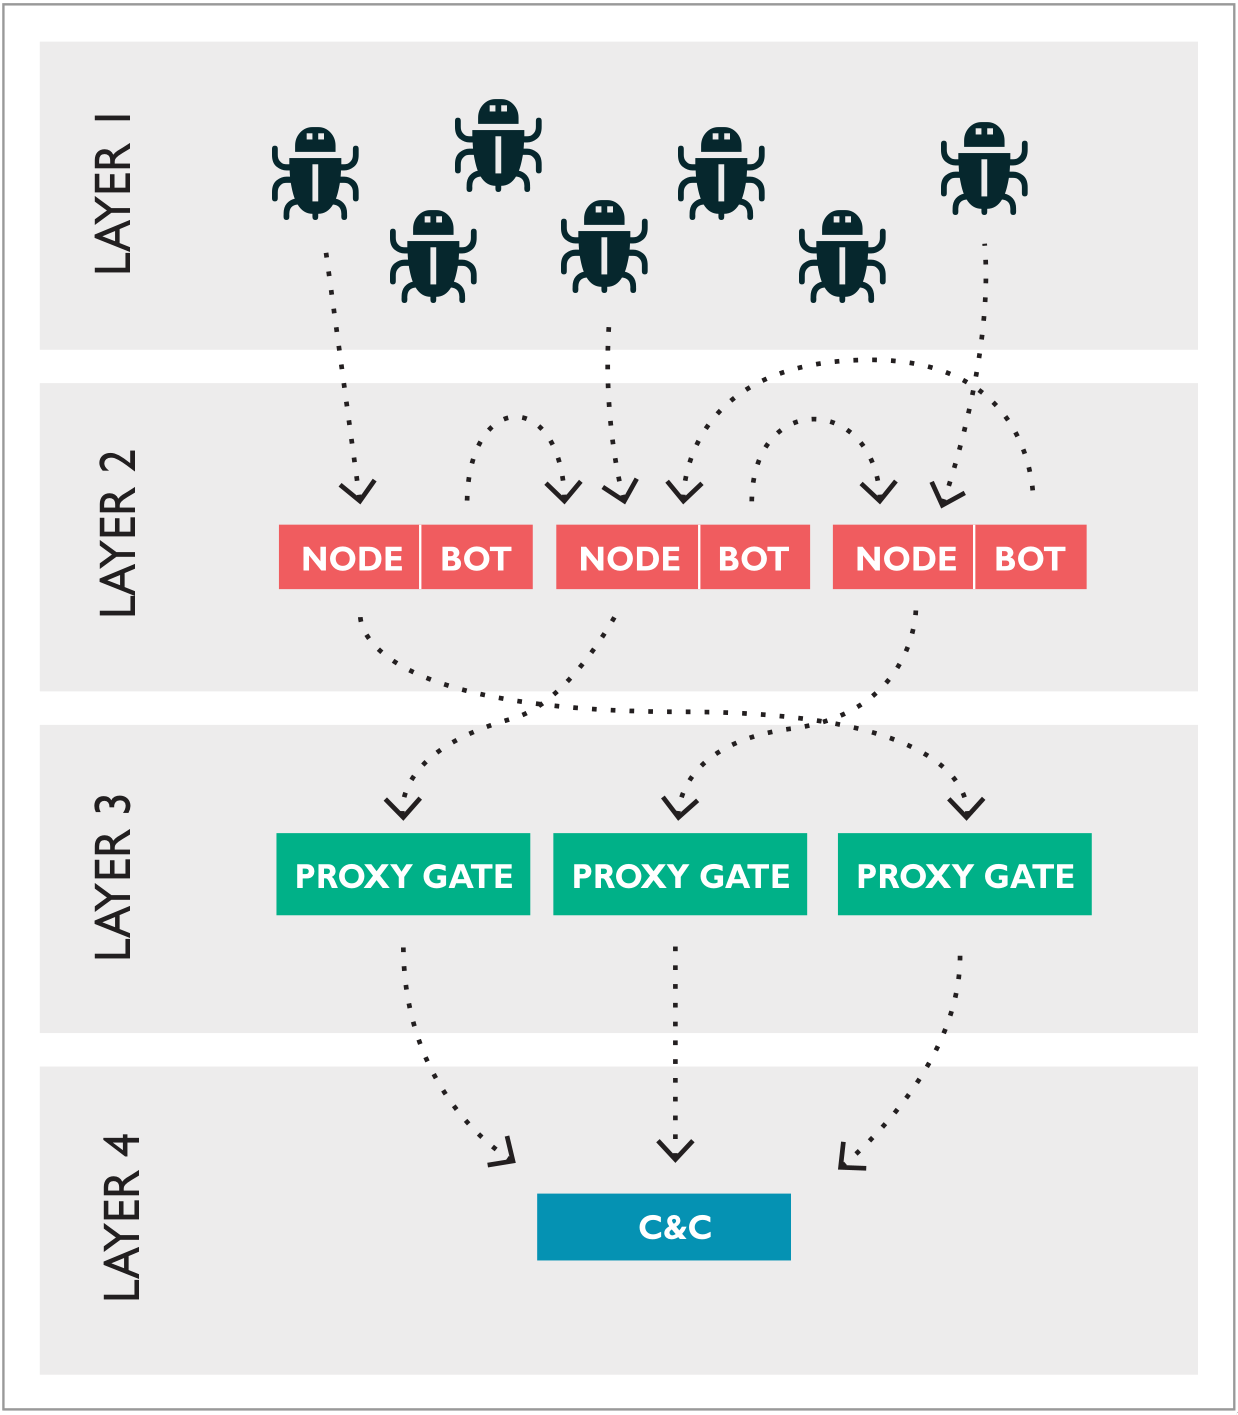
\includegraphics[width=.5\textwidth]{img/dridex_layers}
    \caption[Dridex network layers]{Dridex network layers as described by Blueliv~\cite[Fig. 12]{blueliv2015chasing}\label{fig:Dridex::Network_layers}}
\end{figure}

From a network standpoint, Dridex can be seen as a centralized-\gls{p2p} hybrid \gls{bn}.
It combines \gls{p2p} elements with a strict hierarchy which is atypical for fully decentralized networks.
Additionally, the underlying \gls{p2p} network relies on the hidden \gls{c2} server for orchestration instead of being self-organizing.
As seen in \autoref{fig:Dridex::Network_layers} the \gls{bn} is divided into four main layers starting at the infected machines from layer 1 up to the controlling \gls{c2} server on the fourth layer.
The second layer (L2) is made up of super peers manually elected by the \gls{bm} from the capable \gls{bot} pool, while layer 3 (L3) consists of infected servers which act as proxies to further hide the backend \gls{c2} server~\cite{blueliv2015chasing}.


\section{Reverse engineering\label{sec:Related_work::Reverse_engineering}}
Reverse engineering is a highly iterative process which can be divided into \emph{static} and \emph{dynamic analysis} which are often performed complementary to gain a comprehensive insights on the \gls{mw}'s architecture and behavior.
As the source code is usually not freely available the analyst works with disassembled machine code to reconstruct the high-level behavior.

\begin{description}
    \item[Static analysis] describes the process of tracing the control flow of the assembly code without executing the \gls{mw}.
    The analyst interprets instructions and function calls to determine the purpose of functions or even single blocks.
    This phase often requires significant research on various topics such as operating system \glspl{api}, compiler, and library versions as well as optimizations to decipher the assembly code.
    \item[Dynamic analysis] is performed in a controlled environment where the \gls{mw} gets purposefully executed and monitored.
    This enables the analyst to manipulate execution beyond regular paths by changing register values or skipping instructions.
    Furthermore, resource usage (including network and disk traffic) can be inspected to understand advanced topics such as persistence mechanisms or communication protocols.
\end{description}

Targets of research include communication protocols, membership management, system architecture and general vulnerability analysis.
Successful takedown attempts almost always rely on some sort of weakness in one of these areas~\cite{dittrich2012so}.


\section{Anti-reverse engineering techniques\label{sec:Related_work::Anti_reverse_engineering_techniques}}
As Dridex is a highly successful piece of \gls{mw} we can expect sophisticated obfuscation measures when analyzing the machine code.
The most common technique is \emph{binary packing} which works by applying a mix of compression and encryption to hide the binary from signature based tools.
Yan et al.\ roughly categorize (\gls{mw}) packers in four major categories~\cite{yan2008revealing}.

\begin{description}
    \item[Compressors] are mainly used to reduce file size by applying a regular, off-the-shelf algorithm.
    Although mostly obsolete by modern connection speeds, they are still used today in \gls{mw} and other legitimate use-cases such as archiving and on devices with limited bandwidth.
    Popular compressors are ASPack\fnote{\url{http://www.aspack.com/}} and Ultimate Packer for Executables (UPX)\fnote{\url{https://upx.github.io/}}.
    \item[Crypters] use simple ciphers to prevent the machine code from static analysis.
    As the focus is not on security (the content has to be decrypted eventually anyway) and the \gls{mw} should execute in reasonable time weak algorithms or even simple XORing are commonly chosen.
    \item[Protectors] incorporate techniques from crypters, compressors, and measures to prevent analysis and tampering.
    These include checksums to detect changes in the binary, anti-dumping procedures to hinder direct examination of the malicious code and debugger detection aborting executing in case a debugger is present.
    Besides their use in \gls{mw}, protectors can be found in \gls{drm} applications for instance in the video game industry.
    Themida\fnote{\url{https://www.oreans.com/themida.php}} is a prominent protector.
    \item[Bundlers] produce a single executable containing multiple executable and resource files which unpack themselves in memory only.
    This technique can simplify installation processes and increase usability for the end user.
    Because \gls{mw} often does not require large amounts of raw data besides malicious code they are rarely bundled but regular software (especially targeting non-technical users) may make good use of a bundler.
    An open source example is MoleBox\fnote{\url{https://sudachen.github.io/Molebox/}}.
\end{description}

Breaking packers often involves careful tracking of memory regions (as the decompression/decryption routines are often written to separate allocations first) as well as analysis of the control flow to detect the real entry-point of the \gls{mw}.
After the correct instruction has been reached, execution is stopped, the unpacked executable gets dumped to disk and reloaded into the debugger or disassembler for further analysis.
As packing is often only the first layer of obfuscation the resulting binary may still contain other hurdles such as intentional \emph{dead code}, further \emph{encrypted memory regions} or even complete \emph{virtual machines} which are used to execute the \gls{mw} through custom (or randomized) instruction sets~\cite{you2010malware}.

\section{Summary\label{sec:Related_work::Summary}}
With the recent shift from traditional, centralized \glspl{bn} to \gls{p2p} architectures it becomes even more important to monitor and crawl them to accurately judge the threats they pose.
Dridex is one of the most damaging \glspl{bn} in recent history and has never been openly documented entities making it an ideal target for our research.
The knowledge about its communication protocols and internal architecture could be essential in future takedown attempt.
It is also expected that the \gls{mw} employs several anti-reverse engineering measures which will present a challenge to overcome in the analysis efforts.
